\begin{figure}[htb]
	\centering
	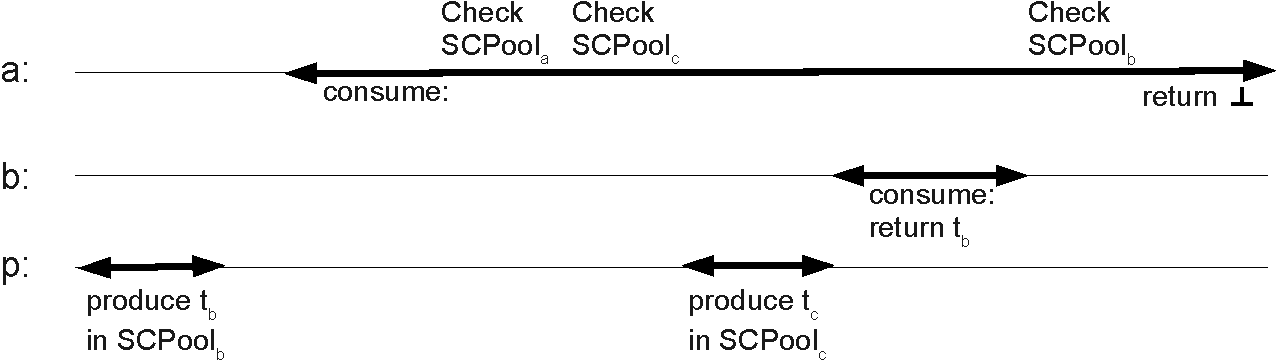
\includegraphics[width=0.7\textwidth]{figures/linearizability-example}
	\caption{\footnotesize{An example where a single traversal may violate linearizability: consumer $a$ is trying to get a task. It fails to take a task from its own pool, and starts looking for chunks to steal in other pools. At this time there is a single non-empty chunk in the system, which is in $b$'s pool; $a$ checks $c$'s pool before $b$'s pool and finds it empty. At this point a producer adds a task to $c$'s pool and then $b$ takes the last task from its pool before $a$ checks it. Thus, $a$ finds $b$'s pool empty, and returns $\bot$. There is no way to linearize this execution, because throughout the execution of $a$'s operation, the system contains at least one task.}}
	\label{fig:linearizability-example}
\end{figure}

\paragraph{Linearizability.}
SALSA pools only return tasks that were inserted to the pool and do not return the same task twice, if a {\bf consume()} or {\bf steal} operation return $\bot$, it does not imply that the pool is empty. For our system to be linearizable we must make sure that it will return $\bot$ if and only if the system contained no tasks during the consume operation. We describe a policy for checking if the system is empty, doing so in a lock-free manner. 

Let us examine why a na\"ive approach, of simply traversing all task pools and returning $\bot$ if no task is found in any of them, violates correctness. First, a consumer might ``miss'' one task added during its traversal, and another removed during the same traversal, as illustrated in Figure 3. In this case, a single traversal would have returned $\bot$ although the pool was not empty at any point during the consume operation. Second, a consumer may miss a task that is moved from one pool to another due to stealing. In order to identify these two cases, we add to each pool a special \emph{emptyIndicator}, a bit array with a bit per-consumer, which is cleared every time the pool may become empty. In SALSA, this occurs when the last task in a chunk is taken or when a chunk is stolen. 
In addition, we implement new function, {\bf checkEmpty()}, which is called by the framework whenever a consumer fails to retrieve tasks from its pool and all other pools. This function ensures that $\bot$ is returned only if there is a time during its execution when there are no tasks in the system. If {\bf checkEmpty()} finds that the pool is not empty, the consumer simply restarts its operation. 

Denote by $c$ the number of consumers in the system. The {\bf checkEmpty()} function works as follows: the consumer traverses the SCPools in the system, to make sure that no tasks are present. After checking a pool, the consumer sets its bit in \emph{emptyIndicator} using a CAS operation. The consumer repeats this traversal $c$ times, where in all traversals except the first, it checks that its bit in \emph{emptyIndicator} is set, i.e., that no chunks were emptied or removed during the traversal. The consumer makes $c$ traversals in order to account for the case that other consumers have already stolen or removed chunks, but did not yet update \emph{emptyIndicator}, and thus their operations were not detected by the consumer. Since up to $c-1$ pending operations by other consumers may begin before any \emph{emptyIndicator} changes, it is guaranteed that after $c$ traversals in which no chunks were seen and the \emph{emptyIndicator} did not change, in one of the traversals the system indeed contains no tasks, and therefore it is safe to return $\bot$. This method is similar to the one used in Concurrent Bags~\cite{Sundell:2011:LAC:1989493.1989550}.
\paragraph{Lock-freedom.}
The operations of every individual SALSA SCPool are trivially wait-free, since they always return. However, a consume operation is restarted whenever {\bf checkEmpty()} returns false, and therefore the algorithm does not guarantee that a consumer will finish every operation. Nevertheless, the system is lock-free, i.e., there always exists some consumer that makes progress. Since 1) whenever all pools are empty for a sufficiently long period, {\bf checkEmpty()} returns true, and 2) a consumer either returns a task or keeps attempting to steal tasks, lock-freedom immediately follows from the following claim:

\begin{claim}
\label{claim:lock-free}
If a consumer returns $\bot$ in $c$ steal attempts from non-empty pools (i.e., pools that contain a task when the steal operation starts), where $c$ is the number of consumers in the system, then at least one consumer in the system returns a task during that time. 
\end{claim}
The proof for this claim appears in Appendix \ref{appendix:lock-freedom}.